\documentclass[11pt]{article}

\usepackage[T1]{fontenc}
\usepackage[utf8]{inputenc}
\usepackage[english]{babel}
\usepackage[margin=1in]{geometry}
\usepackage{lmodern}
\usepackage{microtype}
\usepackage{mathtools}
\usepackage{amsmath,amssymb,amsthm}
\usepackage{array}
\usepackage{booktabs}
\usepackage{tabularx}
\usepackage{float}
\usepackage{graphicx}
\usepackage{caption}
\usepackage{enumitem}
\usepackage{fancyhdr}
\usepackage[numbers]{natbib}
\usepackage{doi}
\usepackage{xurl}
\usepackage{hyperref}
\usepackage{cleveref}
\usepackage{orcidlink}
\usepackage{titling}

\graphicspath{{figures/}}
% Generated by scripts/paper_set_release.py.
% The date is the UTC date when this submission was assembled.
\newif\ifpaperhasdoi
\paperhasdoitrue
\newcommand{\paperdoi}{10.5281/zenodo.22335923}
\newcommand{\manuscriptversion}{Preprint v1.0}
\newcommand{\manuscriptdate}{5 September 2026}
\newcommand{\manuscriptyear}{2026}

\newcommand{\CurrentQ}{Q}
\newcommand{\PredictiveQ}{M}
\newcommand{\Histories}{\mathcal{H}}
\newcommand{\Interfaces}{\mathcal{I}}
\newcommand{\Support}{\Sigma}
\newcommand{\RouteTransport}{\mathfrak{T}}
\newcommand{\CurrentEquiv}{\equiv^{0}}
\newcommand{\FutureEquiv}{\equiv^{+}}


\newtheorem{theorem}{Theorem}[section]
\newtheorem{lemma}[theorem]{Lemma}
\newtheorem{proposition}[theorem]{Proposition}
\newtheorem{corollary}[theorem]{Corollary}
\theoremstyle{definition}
\newtheorem{definition}[theorem]{Definition}
\newtheorem{remark}[theorem]{Remark}
\newtheorem{example}[theorem]{Example}
\newtheorem{convention}[theorem]{Convention}
\floatstyle{ruled}
\newfloat{algorithm}{tbp}{loa}
\floatname{algorithm}{Algorithm}

\urlstyle{same}
\captionsetup{
  font=small,
  labelfont=bf,
  labelsep=period
}
\captionsetup[table]{skip=6pt,position=top}
\captionsetup[figure]{skip=6pt}

\crefname{algorithm}{algorithm}{algorithms}
\Crefname{algorithm}{Algorithm}{Algorithms}
\setlist[enumerate]{leftmargin=*, itemsep=2pt, topsep=4pt}
\setlength{\droptitle}{-3.2em}
\pretitle{\begin{center}\LARGE\bfseries}
\posttitle{\par\end{center}\vspace{0.5em}}
\preauthor{\begin{center}\normalsize}
\postauthor{\par\end{center}\vspace{-0.4em}}
\predate{\begin{center}\small}
\postdate{\par\end{center}\vspace{0.6em}}
\setlength{\emergencystretch}{2em}
\clubpenalty=10000
\widowpenalty=10000
\displaywidowpenalty=10000
\interfootnotelinepenalty=10000
\allowdisplaybreaks[2]
\fancypagestyle{firstpage}{\fancyhf{}
  \fancyfoot[C]{\scriptsize Automorph Inc., Wilmington, DE, USA \quad \texttt{ioannis@automorph.io} \quad \textcopyright\ \manuscriptyear \quad CC-BY 4.0}
  \renewcommand{\headrulewidth}{0pt}
  \renewcommand{\footrulewidth}{0pt}
}

\title{Holonomy with Memory in Six Birds Theory: Predictive Quotients, Witnesses, and Fixed-Support Route Transport}
\author{Ioannis Tsiokos\,\orcidlink{0009-0009-7659-5964}}
\date{\manuscriptdate\\\small\manuscriptversion%
  \ifpaperhasdoi\\\small\href{https://doi.org/\paperdoi}{doi:\paperdoi}\fi}
\hypersetup{
  pdftitle={Holonomy with Memory in Six Birds Theory: Predictive Quotients, Witnesses, and Fixed-Support Route Transport},
  pdfauthor={Ioannis Tsiokos},
  pdfsubject={\manuscriptversion, \manuscriptdate. DOI: \paperdoi},
  hidelinks
}

\begin{document}

\maketitle
\thispagestyle{firstpage}

\begin{abstract}
We introduce a fixed-support route-transport framework in which histories can be equivalent at a current event interface yet differ as predictors of later admissible observations. For each interface, we define a current quotient $\CurrentQ$ by present-event indistinguishability and a predictive quotient $\PredictiveQ$ by equality of all later admissible event statistics under continuation. Standard quotient-algebraic results then apply in this setting: future-predictive equivalence refines current-event equivalence, admissible continuations induce well-defined transport on $\PredictiveQ$, and there is a canonical comparison map $\PredictiveQ \to \CurrentQ$ commuting with transport whenever the continuation also preserves current equivalence. The predictive quotient is future-sufficient, and its projection factors uniquely through the reachable image of every future-sufficient state abstraction. Strict refinement of $\PredictiveQ \to \CurrentQ$ is equivalent to existence of a pair of histories that are current-equivalent but future-distinct, and for endo-continuations, loop action on $\CurrentQ$ can be trivial while loop action on $\PredictiveQ$ is not. The contribution presented here is a specific formulation, mechanization, and exact finite evaluation of these established principles: exact finite fixed-support benchmarks instantiate artifact, flattenable, explicit-latent, dissipative, and coherent-candidate regimes, with bounded robustness under perturbation. Small discovery searches recover additional coherent candidates beyond the hand-built examples while a control search space remains all-flat.
\end{abstract}

\medskip
\noindent\textbf{Keywords:} predictive quotient; fixed support; route transport; loop action; operational equivalence; Six Birds Theory.

\section{Introduction}\label{sec:introduction}
Route dependence is ubiquitous in packaged descriptions of complex systems, but its significance is not always clear. A mismatch between routes may signal no more than bookkeeping, scheduling, or coarse-graining artifacts; equally, it may mark a genuine predictive distinction that is not visible at the current event interface. The central problem of this paper is to separate those cases on a fixed support. We ask when two admissible histories can be indistinguishable by all currently available event tests while still differing as predictors of later admissible observations.

\subsection{Problem statement}\label{subsec:intro-problem}
Six Birds Theory \citep{Tsiokos2026Foundations} is an emergence framework: it constructs a substrate from stable records, package-relative identity, and admissible completion, without importing Hilbert space, amplitudes, or the Born rule. Previous work developed the static event-packaging framework for fixed-support comparison, local event algebras, and admissible global packaging, and showed that contextuality-type obstruction can arise from the substrate's own packaging structure \citep{Tsiokos2026EventPackages}. That obstruction language is adjacent to a broader contextuality literature, from the Kochen--Specker theorem through operational and sheaf-theoretic formulations \citep{KochenSpecker1968ProblemHiddenVariables,Spekkens2005Contextuality,AbramskyBrandenburger2011SheafTheoretic}. The same prior line also sharpened the control lesson that route sensitivity alone is not yet a decisive result: protocol effects may disappear under honest internalization, and some local holonomy may be removable by admissible completion \citep{Tsiokos2026ProtocolTrap,Tsiokos2026FlattenStone}. Route dependence was explicitly demoted from the status of obstruction evidence; it was recognized as diagnostically informative but insufficient on its own.

This raises the question that motivates the present paper: if route dependence on the Six Birds substrate is ubiquitous but not automatically meaningful, what does it actually carry? We study a dynamic route-transport package built on the same fixed-support discipline and ask what predictive structure survives below the current event layer.

The basic distinction is between two equivalence relations at an interface. Histories may be equivalent with respect to the current event package, and they may be equivalent with respect to all later admissible tests under all admissible continuations. Their quotients define a current quotient $\CurrentQ$ and a predictive quotient $\PredictiveQ$. The map $\PredictiveQ \to \CurrentQ$ forgets predictive distinctions not visible at the current interface. Once these definitions are in place, standard quotient-algebraic machinery yields the theorem spine: the predictive quotient is future-sufficient, the predictive projection factors uniquely through the reachable image of every future-sufficient state abstraction, witnesses are equivalent to strict refinement of $\PredictiveQ \to \CurrentQ$, and current-compatible loop actions on the two quotients are intertwined by the comparison map. The individual results are not new in isolation; the contribution is the specific combination of definitions tailored to route transport on fixed support and the demonstration that the resulting framework is non-vacuous.

That demonstration is carried out through exact finite fixed-support models. The benchmark suite separates six operational regimes: flat control, protocol trap, flattenable mismatch, explicit latent memory, dissipative memory, and a coherent-memory candidate. In the coherent-memory benchmark, two histories share one current class but split into two predictive classes, the current loop action is trivial, and the predictive loop action is nontrivial. Robustness sweeps show that the benchmark behaviors survive bounded perturbations in their intended regimes. Bounded discovery searches recover additional coherent candidates beyond the hand-built examples while a control search space remains all-flat.

\subsection{Relation to adjacent literatures}\label{subsec:intro-related}
Equality under all future experiments is a standard state-construction principle. In the deterministic word setting it is the Myhill--Nerode relation: equivalent prefixes remain equivalent after a common suffix, and the resulting quotient yields the minimal observable state construction \citep{Nerode1958LinearAutomatonTransformations}. Our typed observation-valued relation uses the same continuation argument; we do not claim this construction or its minimality as new.

The predictive quotient $\PredictiveQ$ is closest in spirit to future-oriented state constructions such as causal states in computational mechanics, observable operator models, and predictive state representations \citep{ShaliziCrutchfield2001ComputationalMechanics,Jaeger2000ObservableOperatorModels,LittmanSuttonSingh2002PredictiveRepresentationsState}. In all of these frameworks, state is organized by future-observable content rather than by hidden latent memory alone. The present paper does not identify $\PredictiveQ$ with any one of those formalisms. The focus here is a fixed-support formulation of the current/predictive comparison, with explicit compatibility hypotheses, mechanized proofs, and paired finite controls; no priority is claimed for comparing present output with future behavior.

The current and future equivalence relations are also adjacent to behavioral-equivalence and bisimulation traditions in concurrency and probabilistic process theory \citep{Park1981ConcurrencyAutomata,Milner1989CommunicationConcurrency,LarsenSkou1991BisimulationThroughProbabilisticTesting}. Equality of future test values is not, in general, probabilistic bisimulation, which imposes a transition-matching condition. The paper uses observationally defined equivalence relations on typed histories and admissible continuations, and then studies how the corresponding quotients compare.

At the exact finite level, the implementation also sits near classical aggregation and lumpability questions for Markov chains \citep{KemenySnell1976FiniteMarkovChains,Norris1998MarkovChains,Buchholz1994ExactOrdinaryLumpability}. Here again the point is not a new stochastic-kernel formalism. The exact finite machinery is used to realize and audit the quotient comparison rather than to claim a general theory of aggregated stochastic processes.

The comparison itself also has a classical automata interpretation. A deterministic automaton maps a state to its accepted language; evaluating that language at the empty word recovers the current acceptance output, and input transitions act by language derivatives \citep{SilvaEtAl2013GeneralizingDeterminization}. Thus equality of full behavior refines equality of current output, with a canonical map between the resulting quotients. This is the deterministic Boolean-output specialization of our comparison, not a construction first introduced here. The typed interfaces and selected current-compatible continuations specify how we use that pattern.

History $\epsilon$-machines likewise construct states from equality of future distributions and equip them with induced transitions \citep{TraversCrutchfield2011Equivalence}. Links between causal states and bisimulation in partially observable decision processes have also been studied explicitly \citep{ZhangEtAl2019CausalStates}; their stochastic and decision-process assumptions are not asserted for our arbitrary event catalogs. More recently, \citet{BaltieriEtAl2026WorldModels} develop support-restricted predictive models of coupled agent--environment systems, with factorization and induced transition results. Their support is the set of continuations permitted by a coupled process, whereas our fixed support is the declared visible support object. The notions should not be identified, but support-relative predictive comparison and factorization are not exclusive to this paper.

\subsection{Contributions}\label{subsec:intro-contributions}
The contributions of this paper are the following formulation and implementation results, rather than claims of priority for the underlying state-construction principles:
\begin{enumerate}
\item It defines a fixed-support route-transport package with two interface-relative equivalence relations and the associated quotients $\CurrentQ$ and $\PredictiveQ$.
\item It assembles the quotient-algebraic consequences of these definitions into a theorem spine: admissible transport on $\PredictiveQ$, canonicity of the comparison map $\PredictiveQ \to \CurrentQ$, future sufficiency with unique reachable-image factorization, witness equivalence with strict refinement, and loop-action intertwining with an asymmetry theorem. These results specialize established quotient and automata constructions \citep{BurrisSankappanavar1981CourseUniversalAlgebra,Nerode1958LinearAutomatonTransformations}; we claim an explicit assembly and audited examples, not priority for a new quotient or minimal-state theorem.
\item It evaluates the quotient comparison with exact finite benchmarks that separate artifact, flattenable, explicit-latent, dissipative, and coherent-candidate regimes under the same fixed-support discipline.
\item It complements the benchmark suite with bounded robustness checks and conservative discovery searches that show the core signal is not limited to a single hand-built example.
\end{enumerate}

\subsection{Scope and evidence boundary}\label{subsec:intro-scope}
The scope of the paper is deliberately narrow. We do not derive Hilbert-space structure, amplitudes, interference laws, or the Born rule. We do not address Bell-type constraints, nor do we claim a full classification theorem for all route mismatch. The discovery component is bounded and does not establish genericity. What we do claim is more specific: on fixed support, there is a canonical predictive quotient refining the current event quotient, with strictness in the reported non-flat cases, there are exact finite witnesses of strict refinement, and loop action can be trivial on current classes while nontrivial on predictive classes.

\subsection{Guide to the paper}\label{subsec:intro-guide}
Section~\ref{sec:route-transport-packages} defines route transport packages, the two equivalence relations, the current and predictive quotients, and the comparison map. Section~\ref{sec:theorem-spine} states the main theorem spine, including transport, sufficiency, witness, and loop-asymmetry results. Section~\ref{sec:exact-finite-framework} describes the exact finite framework and diagnostics. Sections~\ref{sec:benchmark-suite} and~\ref{sec:controls-robustness} present the benchmark suite, controls, and robustness results. Section~\ref{sec:discovery} summarizes the bounded discovery search and promoted exemplars. Section~\ref{sec:discussion} discusses what has been established and what remains outside the scope of the paper, and Section~\ref{sec:conclusion} concludes. Technical proofs, formal theorem links, computational details, and provenance material are collected in the appendices.

\section{Route Transport Packages and Quotient States}\label{sec:route-transport-packages}
This section fixes the abstract route-transport object used throughout the paper. The point is to distinguish what is visible at a current event interface from what remains relevant for later admissible prediction. We therefore introduce typed histories and continuations on fixed support, define the two interface-relative equivalence relations, and state the quotient-level objects $\CurrentQ$, $\PredictiveQ$, and the comparison map $\PredictiveQ \to \CurrentQ$ that organize the rest of the paper.

\subsection{Fixed support, interfaces, histories, and continuations}\label{subsec:rtp-fixed-support}
We work on a fixed support $\Support$. Throughout the paper, ``fixed support'' means that route comparisons are made on the same comparison base; admissible histories and continuations may carry hidden route information, but they are all interpreted as states of one and the same support object. This is the standing assumption under which the results of the paper are stated.

\begin{definition}[Route transport package]\label{def:route-transport-package}
A route transport package is a typed object
\[
\RouteTransport=
\bigl(
\Support,\Interfaces,\{\Histories_i\}_{i\in\Interfaces},
\{\mathcal{C}_{i\to j}\}_{i,j\in\Interfaces},
\{\mathcal{E}_i\}_{i\in\Interfaces},
\operatorname{id},\operatorname{comp},\operatorname{push},\operatorname{obs}
\bigr)
\]
consisting of the following data:
\begin{enumerate}
\item a fixed support object $\Support$;
\item a family of interfaces $\Interfaces$;
\item for each interface $i\in\Interfaces$, a set $\Histories_i$ of admissible histories terminating at $i$;
\item for each ordered pair $(i,j)$, a set $\mathcal{C}_{i\to j}$ of admissible continuations from $i$ to $j$;
\item for each interface $i$, a set $\mathcal{E}_i$ of admissible events at $i$;
\item identity continuations $1_i\in\mathcal{C}_{i\to i}$ and composition for every composable pair of continuations;
\item a push operation sending $(h,\gamma)\in \Histories_i\times \mathcal{C}_{i\to j}$ to a continued history $\operatorname{push}_{\gamma} h\in\Histories_j$;
\item an observation map assigning to each history-event pair $(h,e)\in\Histories_i\times\mathcal{E}_i$ an observation value $\operatorname{obs}_i(h,e)$.
\end{enumerate}
\end{definition}

An interface is not assumed to be a global time-slice. It is simply a locus at which a stable event package is available. Section~\ref{sec:exact-finite-framework} uses finite catalogs of distributions, kernels, and event packages. Those catalogs need not be closed under composition or push; their quotient maps are checked directly, rather than assumed to instantiate every axiom of the abstract package.

We require
\[
\operatorname{push}_{1_i}h=h,\qquad
\operatorname{push}_{\delta}(\operatorname{push}_{\gamma}h)
=\operatorname{push}_{\delta\circ\gamma}h
\]
for every composable pair. The Lean core records these laws; it does not assume that every later observation is representable by an event available now. Fixed support is a comparison convention in the paper and finite data, not an additional field used by the abstract Lean proofs.

\subsection{Current-event equivalence and future-predictive equivalence}\label{subsec:rtp-equivalences}
The central distinction of the paper is between equivalence at the current event interface and equivalence for all later admissible purposes. Let $i\in\Interfaces$ and let $h,h'\in\Histories_i$.

\begin{definition}[Current-event equivalence]\label{def:current-event-equivalence}
Histories $h$ and $h'$ are current-event equivalent at interface $i$, written
\[
h \CurrentEquiv_i h',
\]
iff they agree on all current admissible events:
\begin{equation}
h \CurrentEquiv_i h'
\quad\Longleftrightarrow\quad
\forall e\in\mathcal{E}_i,\;
\operatorname{obs}_i(h,e)=\operatorname{obs}_i(h',e).
\label{eq:current-equivalence}
\end{equation}
\end{definition}

This is the ``same now'' relation determined by the current event package.

\begin{definition}[Future-predictive equivalence]\label{def:future-predictive-equivalence}
Histories $h$ and $h'$ are future-predictively equivalent at interface $i$, written
\[
h \FutureEquiv_i h',
\]
iff they agree on all later admissible event observations after all admissible continuations:
\begin{equation}
h \FutureEquiv_i h'
\quad\Longleftrightarrow\quad
\forall j\in\Interfaces\;\forall \gamma\in\mathcal{C}_{i\to j}\;\forall e\in\mathcal{E}_j,\;
\operatorname{obs}_j(\operatorname{push}_{\gamma} h,e)
=
\operatorname{obs}_j(\operatorname{push}_{\gamma} h',e).
\label{eq:future-equivalence}
\end{equation}
\end{definition}

This is the ``same for all later admissible purposes'' relation. Conceptually, it is closest to future-oriented state constructions such as observable operator models, predictive state representations, and causal-state partitions \citep{Jaeger2000ObservableOperatorModels,LittmanSuttonSingh2002PredictiveRepresentationsState,ShaliziCrutchfield2001ComputationalMechanics}. At a more abstract level it is also adjacent to behavioral-equivalence and probabilistic-bisimulation traditions \citep{Milner1989CommunicationConcurrency,LarsenSkou1991BisimulationThroughProbabilisticTesting}. In later sections we will show that it refines current-event equivalence and therefore defines a strictly richer quotient whenever predictive distinctions survive below current event resolution.

\begin{definition}[Current-compatible continuation]\label{def:current-compatible}
A continuation $\gamma\in\mathcal{C}_{i\to j}$ is current-compatible if
\[
h\CurrentEquiv_i h'\ \Longrightarrow\
\operatorname{push}_{\gamma}h\CurrentEquiv_j\operatorname{push}_{\gamma}h'.
\]
This is a condition on a selected continuation, not an axiom on the entire catalog.
\end{definition}

If every continuation were current-compatible, current equivalence would imply future equivalence. Together with the identity law this would make the two relations equal and rule out predictive witnesses. In particular, a universal event-pullback law into the present event package is too strong for the non-flat examples. A readout may reveal a distinction that a current-compatible loop transports without revealing.

\subsection{The current quotient \texorpdfstring{$\CurrentQ$}{Q} and predictive quotient \texorpdfstring{$\PredictiveQ$}{M}}\label{subsec:rtp-quotients}
The two equivalence relations define two interface-relative state objects in the ordinary quotient sense \citep{MacLaneBirkhoff1999Algebra,BurrisSankappanavar1981CourseUniversalAlgebra}:
\begin{equation}
\CurrentQ_i := \Histories_i / \CurrentEquiv_i,
\qquad
\PredictiveQ_i := \Histories_i / \FutureEquiv_i.
\label{eq:quotients}
\end{equation}

The quotient $\CurrentQ_i$ is the current event state at interface $i$: it identifies histories that cannot be distinguished by the current event package. The quotient $\PredictiveQ_i$ is the predictive state at interface $i$: it identifies histories only when no admissible continuation and later event can distinguish them.

The asymmetry between these two quotients is the main structural phenomenon of the paper. Theorem~\ref{thm:future-refines-current} will show that future-predictive equivalence refines current-event equivalence. Consequently, the identity on histories descends to a canonical comparison map
\begin{equation}
\pi_i : \PredictiveQ_i \to \CurrentQ_i.
\label{eq:comparison-map}
\end{equation}

For $q\in\CurrentQ_i$, the fiber $\pi_i^{-1}(q)$ is the predictive residue hidden below one current class. In the exact finite framework of Section~\ref{sec:exact-finite-framework}, the largest such multiplicity appears as the max-fiber diagnostic used throughout the benchmark and discovery results.

\subsection{The comparison map \texorpdfstring{$\PredictiveQ \to \CurrentQ$}{M to Q}}\label{subsec:rtp-comparison}
The strictness of the comparison map is witnessed directly at the level of histories.

\begin{definition}[Predictive witness]\label{def:predictive-witness}
A predictive witness at interface $i$ is a pair of histories $h,h'\in\Histories_i$ such that
\begin{equation}
h \CurrentEquiv_i h'
\qquad\text{and}\qquad
\neg\bigl(h \FutureEquiv_i h'\bigr).
\label{eq:predictive-witness}
\end{equation}
\end{definition}

A predictive witness says that one current class contains more than one predictive class. Section~\ref{sec:theorem-spine} turns this informal statement into a quotient-level strict-refinement theorem.

We also fix the paper's loop notation here. A loop at interface $i$ is an admissible endo-continuation $\ell\in\mathcal{C}_{i\to i}$. At the level of representatives, a loop acts by
\begin{equation}
h \longmapsto \operatorname{push}_{\ell} h.
\label{eq:loop-representative-action}
\end{equation}
For a loop that preserves current equivalence, Section~\ref{sec:theorem-spine} proves that this representative action descends to well-defined endomorphisms
\[
L^{\PredictiveQ}_{\ell} : \PredictiveQ_i \to \PredictiveQ_i,
\qquad
L^{\CurrentQ}_{\ell} : \CurrentQ_i \to \CurrentQ_i,
\]
and that the comparison map intertwines them. The target asymmetry studied later is exactly the situation in which $L^{\CurrentQ}_{\ell}$ is trivial while $L^{\PredictiveQ}_{\ell}$ is not.

\section{Theorem Spine}\label{sec:theorem-spine}
The results in this section form the abstract theorem spine. Each is a standard consequence of the definitions in Section~\ref{sec:route-transport-packages}; the value of stating them explicitly is to fix the precise quotient-level structure used to interpret the benchmark suite, subject to the finite-catalog checks in Section~\ref{sec:exact-finite-framework} and to anchor the Lean formalization. The results do not depend on the exact finite implementation of later sections. For transparency, Table~\ref{tab:theorem-lean-map} records the principal Lean theorem names supporting each result; Appendix~\ref{app:lean-core} returns to that formal map in more detail.

\begin{table}[H]
\centering
\caption{Main theorem statements and their primary Lean counterparts.}
\label{tab:theorem-lean-map}
\footnotesize
\setlength{\tabcolsep}{4pt}
\resizebox{\linewidth}{!}{%
\begin{tabular}{@{}ll@{}}
\toprule
Paper statement & Primary Lean name(s) \\
\midrule
Theorem~\ref{thm:future-refines-current} &
\nolinkurl{futurePredictiveEquiv_implies_currentEventEquiv} \\
Theorem~\ref{thm:predictive-transport} &
\begin{tabular}[t]{@{}l@{}}
\nolinkurl{futurePredictiveEquiv_push} \\
\nolinkurl{predictiveToCurrent_commutes_with_transport}
\end{tabular} \\
Theorem~\ref{thm:future-sufficient} &
\nolinkurl{predictiveQuotient_futureSufficient} \\
Theorem~\ref{thm:reachable-factorization} &
\begin{tabular}[t]{@{}l@{}}
\nolinkurl{futureSufficient_factorsThroughPredictiveQuotient_onReachable} \\
\nolinkurl{futureSufficient_factorization_unique_onReachable}
\end{tabular} \\
Theorem~\ref{thm:witness-strict-refinement} &
\nolinkurl{strictRefinement_iff_nonempty_predictiveWitness} \\
Theorem~\ref{thm:loop-asymmetry} &
\begin{tabular}[t]{@{}l@{}}
\nolinkurl{predictiveToCurrent_commutes_with_loopAction} \\
\nolinkurl{loopAsymmetry_exhibits_movedPredictive_fixedCurrent}
\end{tabular} \\
\bottomrule
\end{tabular}}
\end{table}

\subsection{Future equivalence refines current equivalence}\label{subsec:thm-refinement}
\begin{theorem}\label{thm:future-refines-current}
For every interface $i$, future-predictive equivalence refines current-event equivalence:
\[
h \FutureEquiv_i h'
\quad\Longrightarrow\quad
h \CurrentEquiv_i h'
\qquad
(h,h'\in\Histories_i).
\]
Consequently, the identity on histories descends to a canonical comparison map
\[
\pi_i : \PredictiveQ_i \to \CurrentQ_i.
\]
\end{theorem}

\paragraph{Proof sketch.}
Take the identity continuation at interface $i$ in the definition of future-predictive equivalence. The required equalities then reduce to equality of current event observations, yielding current-event equivalence. The Lean theorem \nolinkurl{futurePredictiveEquiv_implies_currentEventEquiv} formalizes this refinement. The comparison map is the standard descent from a finer equivalence relation to a coarser one \citep{BurrisSankappanavar1981CourseUniversalAlgebra}.

\subsection{Predictive transport under continuation}\label{subsec:thm-transport}
\begin{theorem}\label{thm:predictive-transport}
For every admissible continuation $\gamma\in\mathcal{C}_{i\to j}$, pushing representatives descends to a predictive transport map. If $\gamma$ is current-compatible in the sense of Definition~\ref{def:current-compatible}, it also descends to a current transport map:
\[
T^{\PredictiveQ}_{\gamma} : \PredictiveQ_i \to \PredictiveQ_j,
\qquad
T^{\CurrentQ}_{\gamma} : \CurrentQ_i \to \CurrentQ_j.
\]
Moreover, these transport maps are intertwined by the comparison map:
\[
\pi_j \circ T^{\PredictiveQ}_{\gamma}
=
T^{\CurrentQ}_{\gamma} \circ \pi_i.
\]
\end{theorem}

\paragraph{Proof sketch.}
Future-predictive equivalence is preserved by pushing along an admissible continuation, so continuation induces a well-defined map on predictive classes. Current-event equivalence is preserved by the additional current-compatibility hypothesis on this continuation, so it also induces a map on current classes. This hypothesis is not imposed on every admissible continuation. The predictive argument is the right-congruence argument of automata theory, and the descent step is the usual quotient construction \citep{Nerode1958LinearAutomatonTransformations,BurrisSankappanavar1981CourseUniversalAlgebra}. No probabilistic bisimulation theorem is being invoked. When current compatibility holds, the comparison map commutes with the two induced maps because both descend from the same representative push operation. In Lean, the predictive well-definedness theorem is \nolinkurl{futurePredictiveEquiv_push}, and the quotient-level commutation statement is \nolinkurl{predictiveToCurrent_commutes_with_transport}.

\subsection{Future sufficiency of the predictive quotient}\label{subsec:thm-sufficiency}
\begin{theorem}\label{thm:future-sufficient}
For every interface $i$, the canonical map from histories to predictive classes,
\[
h \longmapsto [h]_{\FutureEquiv_i},
\]
is future-sufficient: every future observable at $i$ factors through the predictive quotient $\PredictiveQ_i$. Here a state map $s:\Histories_i\to S$ is future-sufficient when for each continuation-event pair there is a function $g:S\to\mathcal{O}$ with $\operatorname{obs}_j(\operatorname{push}_{\gamma}h,e)=g(s(h))$ for every history, where $\mathcal{O}$ is the observation codomain. This is set-theoretic factorization; no statistical model family or conditional-distribution sufficiency is asserted.
\end{theorem}

\paragraph{Proof sketch.}
A future observable is determined by a target interface, an admissible continuation, and a later admissible event. By definition of future-predictive equivalence, such an observable is constant on each predictive class. Hence it descends to a well-defined function on $\PredictiveQ_i$. This set-theoretic descent is analogous to sufficient-statistic factorization and predictive-state constructions; it does not invoke the probabilistic hypotheses of classical sufficiency theory \citep{LehmannCasella1998TheoryPointEstimation,Jaeger2000ObservableOperatorModels,ShaliziCrutchfield2001ComputationalMechanics}. The Lean theorem \nolinkurl{predictiveQuotient_futureSufficient} formalizes exactly this quotient-level sufficiency statement.

\subsection{Reachable-image factorization and uniqueness}\label{subsec:thm-factorization}
\begin{theorem}\label{thm:reachable-factorization}
Let $s : \Histories_i \to S$ be any future-sufficient state abstraction at interface $i$. Then on the reachable image
\[
\operatorname{Reach}(s) := \{\,s(h) : h\in\Histories_i\,\},
\]
there exists a factor map
\[
f : \operatorname{Reach}(s) \to \PredictiveQ_i
\]
such that
\[
f(s(h)) = [h]_{\FutureEquiv_i}
\qquad
\text{for all } h\in\Histories_i.
\]
Moreover, this factorization is unique on the reachable image: if two maps from $\operatorname{Reach}(s)$ to $\PredictiveQ_i$ agree with the predictive quotient on all histories, then they agree everywhere on $\operatorname{Reach}(s)$.
\end{theorem}

\paragraph{Proof sketch.}
Future sufficiency implies that histories with the same state value under $s$ must be future-predictively equivalent. Thus the predictive quotient depends only on the reachable state value, giving a well-defined factor map on $\operatorname{Reach}(s)$. At the mathematical level, this is a reachable-image factorization through the kernel of a sufficient state map in the standard algebraic and statistical sense \citep{BurrisSankappanavar1981CourseUniversalAlgebra,LehmannCasella1998TheoryPointEstimation}. Uniqueness follows because every reachable state has at least one representing history, and both candidate factor maps are required to agree on those representatives. The Lean existence theorem is \nolinkurl{futureSufficient_factorsThroughPredictiveQuotient_onReachable}; the corresponding uniqueness theorem is \nolinkurl{futureSufficient_factorization_unique_onReachable}.

\subsection{Witness objects and strict refinement}\label{subsec:thm-witnesses}
\begin{theorem}\label{thm:witness-strict-refinement}
At a fixed interface $i$, the following are equivalent:
\begin{enumerate}
\item the comparison map $\pi_i : \PredictiveQ_i \to \CurrentQ_i$ is strictly refining, in the sense that there exist distinct predictive classes with the same current image;
\item there exists a predictive witness at $i$, that is, histories $h,h'\in\Histories_i$ such that
\[
h \CurrentEquiv_i h'
\qquad\text{and}\qquad
\neg\bigl(h \FutureEquiv_i h'\bigr).
\]
\end{enumerate}
\end{theorem}

\paragraph{Proof sketch.}
A predictive witness immediately gives two different predictive classes whose images in $\CurrentQ_i$ coincide, so it yields strict refinement of $\pi_i$. Conversely, if $\pi_i$ identifies two distinct predictive classes, choose representatives of those classes; their current images agree while their predictive classes remain distinct, giving a witness. This is the representative-level criterion for noninjectivity of the comparison map, using ordinary quotient equality \citep{MacLaneBirkhoff1999Algebra}. The Lean equivalence theorem is \nolinkurl{strictRefinement_iff_nonempty_predictiveWitness}, with the forward and backward directions also available separately through the witness module.

\subsection{Loop action and asymmetry}\label{subsec:thm-loops}
\begin{theorem}\label{thm:loop-asymmetry}
Let $\ell\in\mathcal{C}_{i\to i}$ be a current-compatible loop at interface $i$. Then $\ell$ induces endomorphisms
\[
L^{\PredictiveQ}_{\ell} : \PredictiveQ_i \to \PredictiveQ_i,
\qquad
L^{\CurrentQ}_{\ell} : \CurrentQ_i \to \CurrentQ_i,
\]
and these are intertwined by the comparison map:
\[
\pi_i \circ L^{\PredictiveQ}_{\ell}
=
L^{\CurrentQ}_{\ell} \circ \pi_i.
\]
In particular, if $L^{\CurrentQ}_{\ell}$ is trivial while $L^{\PredictiveQ}_{\ell}$ is nontrivial, then there exists a predictive class $q\in\PredictiveQ_i$ such that
\[
L^{\PredictiveQ}_{\ell}(q)\neq q
\qquad\text{but}\qquad
\pi_i\bigl(L^{\PredictiveQ}_{\ell}(q)\bigr)=\pi_i(q).
\]
\end{theorem}

\paragraph{Proof sketch.}
Loop action is the endomorphism specialization of continuation transport, so the quotient actions are inherited from the transport constructions already established above. The intertwining identity is the loop-specialized form of the transport commutation theorem. If the current action is trivial and the predictive action is not, choose a predictive class moved by the loop. Intertwining then forces its current image to remain fixed. In Lean, the quotient-level commutation theorem is \nolinkurl{predictiveToCurrent_commutes_with_loopAction}, and the existential asymmetry theorem is \nolinkurl{loopAsymmetry_exhibits_movedPredictive_fixedCurrent}.

The last implication is an elementary consequence of an intertwining map, not a new general theorem about actions. Here ``loop'' means an endo-continuation; neither geometric holonomy nor a connection or curvature is constructed.

\section{Exact Finite Framework}\label{sec:exact-finite-framework}
This section specifies the exact finite framework used for all computational results in the paper. The computation uses finite typed catalogs with exact rational arithmetic. The abstract package of Section~\ref{sec:route-transport-packages} supplies sufficient conditions for quotient descent; finite-catalog descent is checked separately as described below. Histories are rational distributions on finite internal state sets, admissible continuations are rational row-stochastic kernels, and event packages are rational observables on visible support. The quotient constructions and diagnostics reported later are therefore exact finite invariants of the declared model rather than floating-point approximations.

\subsection{Exact finite route-transport packages}\label{subsec:eff-packages}
Fix a finite support label set $\Sigma$ and a finite interface set $\Interfaces$. For each interface $i\in\Interfaces$, an exact finite route-transport package specifies:
\begin{enumerate}
\item a finite internal state set $X_i$;
\item a support projection
\[
p_i : X_i \to \Sigma;
\]
\item a finite declared history set $\Histories_i$, where each history $h\in\Histories_i$ is a rational probability distribution on $X_i$;
\item for each ordered pair $(i,j)$, a finite continuation set $\mathcal{C}_{i\to j}$, where each $\gamma\in\mathcal{C}_{i\to j}$ is a rational row-stochastic kernel
\[
K_{\gamma} : X_i \times X_j \to \mathbb{Q}_{\ge 0};
\]
\item a finite event package $\mathcal{E}_i$, where each event $e\in\mathcal{E}_i$ is represented by a rational weight function
\[
w_e : \Sigma \to \mathbb{Q}.
\]
\end{enumerate}

Histories are treated as row vectors. For $h\in\Histories_i$ and $\gamma\in\mathcal{C}_{i\to j}$, the continued history is
\begin{equation}
\bigl(\operatorname{push}_{\gamma} h\bigr)(y)
=
\sum_{x\in X_i} h(x)\,K_{\gamma}(x,y),
\qquad y\in X_j.
\label{eq:finite-push}
\end{equation}
Current event observations are computed by first projecting internal states to visible support and then applying the event weights:
\begin{equation}
\operatorname{obs}_i(h,e)
=
\sum_{x\in X_i} h(x)\,w_e\!\bigl(p_i(x)\bigr).
\label{eq:finite-observation}
\end{equation}

The implementation uses exact rational arithmetic throughout. In particular, no benchmark, control, robustness run, or discovery candidate depends on floating-point equality at the quotient-computation layer.
The finite-state kernel language used here is standard in the theory of finite Markov chains \citep{Norris1998MarkovChains}. The runtime uses one common internal state set and support projection across interfaces, a special case of the indexed notation above. Declared histories need not be closed under push.

\subsection{Signatures, partitions, and quotient computation}\label{subsec:eff-signatures}
At a fixed interface $i$, all quotient computations are performed on the declared history set $\Histories_i$ in its declared order. The current signature of a history is the ordered vector of all current event observations:
\begin{equation}
s_i^{0}(h)
:=
\bigl(\operatorname{obs}_i(h,e)\bigr)_{e\in\mathcal{E}_i}.
\label{eq:current-signature}
\end{equation}
The future signature of a history is the ordered vector of all later event observations after all declared admissible continuations out of $i$:
\begin{equation}
s_i^{+}(h)
:=
\bigl(
\operatorname{obs}_j(\operatorname{push}_{\gamma} h,e)
\bigr)_{(\gamma,e)\in\mathcal{F}_i},
\label{eq:future-signature}
\end{equation}
where $\mathcal{F}_i$ is the declared ordered list of all pairs $(\gamma,e)$ such that $\gamma\in\mathcal{C}_{i\to j}$ for some target interface $j$ and $e\in\mathcal{E}_j$.

Two histories are placed in the same current class exactly when their current signatures agree, and they are placed in the same predictive class exactly when their future signatures agree. Thus the exact finite quotients $\CurrentQ_i$ and $\PredictiveQ_i$ are computed by exact equality of signature vectors. The implementation does not insert any transitive closure or derived continuation family at this stage: the future signature is computed only from the declared admissible continuation catalog of the benchmark or discovered candidate.

The machine-readable artifacts record the resulting interface counts directly. In particular:
\begin{itemize}
\item \texttt{history\_count} records $|\Histories_i|$;
\item \texttt{current\_quotient\_size} records $|\CurrentQ_i|$;
\item \nolinkurl{predictive_quotient_size} records $|\PredictiveQ_i|$.
\end{itemize}
A comparison map requires that the predictive partition refine the current partition. Identity experiments imply this in the abstract core; for finite catalogs it must hold for the declared signatures and is checked in the finalization audit at every reported benchmark interface and discovery primary interface. The terminal discovery exceptions are stated in Section~\ref{subsec:discovery-spaces}; no comparison map is asserted there. These fields count the quotients of the declared finite history set. They do not assert equivalence under unlisted continuation sequences. For each reported transport, the implementation checks that every pushed source member has the signature of a declared target class and that all members of one source class land in the same target class. A missing target signature or a split class raises an error. These finite checks provide quotient maps on the tested catalogs; they are not a proof that the catalogs satisfy the composition and history-closure assumptions of the abstract core.
The broader background for finite-state aggregation questions is the classical lumpability literature for Markov chains, although the present quotients are defined by event signatures rather than by preservation of the Markov property under aggregation \citep{KemenySnell1976FiniteMarkovChains,Buchholz1994ExactOrdinaryLumpability}.

\subsection{Diagnostics}\label{subsec:eff-diagnostics}
Four interface-level diagnostics organize the benchmark and discovery results.

First, the \emph{witness count} is the number of unordered pairs of declared histories in one current class but in different predictive classes. This is the exact finite count of predictive witnesses at the chosen interface.

Second, the \emph{max fiber size} records the largest multiplicity of predictive classes above a single current class:
\begin{equation}
\operatorname{MaxFiber}_i
:=
\max_{q\in\CurrentQ_i}
\#\bigl(\pi_i^{-1}(q)\bigr).
\label{eq:max-fiber}
\end{equation}
In the artifact outputs this appears as \texttt{max\_fiber\_size}. The maximum is taken as zero for an empty history set. Likewise, the discrepancy and maximum loop scores below are zero when there are no tested pairs, future tests, or loops, respectively.

Third, we use an exact discrepancy metric that measures the largest later predictive mismatch hidden inside one current class. For a fixed interface $i$, define
\begin{equation}
\Delta_i^{\max}
:=
\max_{\substack{h,h'\in\Histories_i\\ h \CurrentEquiv_i h'}}
\;
\max_{\substack{j\in\Interfaces\\ \gamma\in\mathcal{C}_{i\to j}\\ e\in\mathcal{E}_j}}
\left|
\operatorname{obs}_j(\operatorname{push}_{\gamma} h,e)
-
\operatorname{obs}_j(\operatorname{push}_{\gamma} h',e)
\right|.
\label{eq:exact-max-gap}
\end{equation}
This is the exact finite implementation of the predictive-sufficiency deficit used in the repo \citep{Tsiokos2026CastStone}. In the machine-readable outputs, the metric name is recorded as \nolinkurl{exact_max_abs_future_gap} and its value appears under \nolinkurl{discrepancy_metric_value}.

Fourth, loop action is summarized by moved-class fractions on the current and predictive quotients. For a tested loop $\ell\in\mathcal{C}_{i\to i}$, let
\[
L^{\CurrentQ}_{\ell} : \CurrentQ_i \to \CurrentQ_i,
\qquad
L^{\PredictiveQ}_{\ell} : \PredictiveQ_i \to \PredictiveQ_i
\]
be the induced quotient endomorphisms. The exact finite loop score at interface $i$ is the fraction of quotient classes moved by the loop action. The per-interface artifact values
\nolinkurl{loop_action_score_current_quotient}
and
\nolinkurl{loop_action_score_predictive_quotient}
are defined as the maximum moved-class fraction over the loops explicitly listed for that benchmark or candidate at that interface.

\subsection{Controls and admissibility checks}\label{subsec:eff-controls}
The implementation assigns labels by a fixed precedence rule: an artifact flag, flatness, a passed flattening check, a passed currentization check, a dissipative flag, and finally a residual candidate label. Artifact and dissipative flags are supplied by the benchmark manifest. The candidate label alone does not assert nontrivial loop action or successful support checks; those quantities must be read separately. The six examples therefore illustrate operational readings, not a classifier proven to characterize six intrinsic classes.

The computational framework is paired with explicit control logic. The purpose of these controls is to separate route-sensitive effects that survive fixed-support comparison from those that disappear under admissible repair.

The first control is \emph{support fixation}. When two models are compared as a pair, the visible support surface is checked explicitly. A same-support-required comparison fails if the paired models do not agree on the declared visible support labels. The corresponding machine-readable field is \nolinkurl{support_fixation_status}.

The second control is \emph{completion} or \emph{flattening}. In a designated base/completed pair, the completion status is positive only when the base model is non-flat and the completed model collapses the effect at the compared interface. Operationally, the completed side must have zero witnesses and zero discrepancy; the reported completed benchmark has $|\CurrentQ_i|=|\PredictiveQ_i|$. This is a designated-pair check, not an algorithm that finds or certifies every admissible completion. This status is recorded as \nolinkurl{flattening_status}.

The third control is \emph{currentization}. In a designated base/refined pair, the currentization status is positive only when predictive residue present in the base model becomes current-visible and therefore disappears as hidden predictive structure in the refined model. The implemented currentization predicate checks base residue and zero witnesses and discrepancy on the refined side; the reported refined benchmark also has max fiber size one. It does not independently prove that the change is a refinement morphism. This status is recorded as \texttt{currentization\_status}.

Finally, bounded perturbation robustness is evaluated by benchmark-specific survival predicates under deterministic perturbation bundles that preserve the structural shape of the model. The resulting survival fraction is recorded as \texttt{robustness\_fraction}. The benchmark and discovery sections use these control and robustness ledgers directly rather than introducing any additional informal acceptance criteria.

\section{Benchmark Suite}\label{sec:benchmark-suite}
This section presents the benchmark suite. The first half is intentionally control-heavy: before turning to dissipative transport and loop asymmetry, we separate four operational situations that can otherwise be conflated in route-sensitive data. The flat control provides the zero-memory baseline; the protocol-trap pair shows that apparent route significance can disappear under honest internalization; the flattenable pair shows that some mismatch is removable by admissible completion; and the explicit latent-memory pair isolates hidden predictive residue that becomes current-visible under same-support refinement. Table~\ref{tab:bench-control-family} collects the exact interface-level metrics for this first benchmark family, and Table~\ref{tab:bench-control-pairs} summarizes the paired-control readings.

\begin{table}[H]
\centering
\caption{Exact interface-level metrics for the control-heavy benchmark family at the measured interface \texttt{mid}.}
\label{tab:bench-control-family}
\footnotesize
\setlength{\tabcolsep}{4pt}
\resizebox{\linewidth}{!}{%
\begin{tabular}{@{}llcccccl@{}}
\toprule
Benchmark & Role & $|\CurrentQ|$ & $|\PredictiveQ|$ & Max fiber & Wit. & Gap & Label \\
\midrule
\nolinkurl{flat_control} & flat baseline & 1 & 1 & 1 & 0 & 0 & flat \\
\nolinkurl{protocol_trap_naive} & naive route-sensitive case & 1 & 2 & 2 & 1 & 1 & artifact\_trap \\
\nolinkurl{protocol_trap_honest} & honest control & 1 & 1 & 1 & 0 & 0 & flat \\
\nolinkurl{flattenable_raw} & raw mismatch & 1 & 2 & 2 & 1 & 1 & flattenable \\
\nolinkurl{flattenable_completed} & completed counterpart & 1 & 1 & 1 & 0 & 0 & flat \\
\nolinkurl{latent_memory_base} & base latent case & 1 & 2 & 2 & 1 & 1 & explicit\_latent \\
\nolinkurl{latent_memory_refined} & refined currentized case & 2 & 2 & 1 & 0 & 0 & flat \\
\bottomrule
\end{tabular}}
\end{table}

\subsection{Flat control}\label{subsec:bench-flat}
The flat control is the baseline for the entire benchmark suite. At the measured interface \texttt{mid}, the benchmark has two declared histories but only one current class and one predictive class. The witness count is zero, the max fiber size is one, the exact discrepancy metric is zero, and both loop-action scores vanish. In the machine-readable outputs this benchmark is classified \texttt{flat}; operationally, that classification is an exact statement about the declared event package and continuation catalog.

This benchmark matters because the later non-flat cases are interpreted against it rather than against an informal expectation that route sensitivity is automatically meaningful. The flat control shows what the quotient comparison looks like when no predictive residue survives below current event resolution. In particular, the benchmark exhibits neither strict refinement of $\PredictiveQ \to \CurrentQ$ nor any hidden multiplicity inside current classes.

\subsection{Protocol-trap pair}\label{subsec:bench-protocol-trap}
The protocol-trap pair is designed to show that non-flat route sensitivity need not survive honest protocol internalization, in line with the artifact logic developed in \citep{Tsiokos2026ProtocolTrap}. In the naive benchmark, the measured interface \texttt{mid} has $|\CurrentQ|=1$, $|\PredictiveQ|=2$, max fiber size $2$, witness count $1$, discrepancy $1$, and classification \texttt{artifact\_trap}. The same-support check used by the pairwise comparison is non-failing, so the paired interpretation does not rely on changing the support object between the two models.

The honest/internalized counterpart is flat at the same interface: $|\CurrentQ|=|\PredictiveQ|=1$, max fiber size $1$, witness count $0$, discrepancy $0$, and both loop-action scores $0$. The paired-control outcome is therefore specific and limited: this benchmarked route-sensitive effect disappears once the relevant bookkeeping is internalized honestly. We do not infer from this pair that every route-sensitive effect is an artifact. We infer only that route sensitivity by itself is not enough, and that the present naive example falls on the artifact side of that line.

\subsection{Flattenable pair}\label{subsec:bench-flattenable}
The flattenable pair separates removable mismatch from transported predictive residue and mirrors the completion logic studied in \citep{Tsiokos2026FlattenStone}. In the raw benchmark, the measured interface \texttt{mid} is non-flat with $|\CurrentQ|=1$, $|\PredictiveQ|=2$, max fiber size $2$, witness count $1$, discrepancy $1$, and class label \texttt{flattenable}. The same-support comparison is non-failing and the designated completion control returns a positive \texttt{flattening\_status}.

The completed counterpart collapses the effect: at \texttt{mid} it has $|\CurrentQ|=|\PredictiveQ|=1$, max fiber size $1$, witness count $0$, discrepancy $0$, and both loop-action scores $0$. This is the operational content of flattenability in the present paper. The raw model is not classified as a protocol artifact, because the relevant repair here is admissible completion on fixed support rather than honest protocol internalization. What matters is that the mismatch is removable by the specified completion and therefore does not force a persistent predictive quotient beyond the completed presentation.

\subsection{Explicit latent-memory pair}\label{subsec:bench-explicit-latent}
The explicit latent-memory pair is the first benchmark in which hidden predictive residue is retained as a positive phenomenon rather than dismissed as artifact or removable mismatch, and it plays the same-support refinement role anticipated by the fixed-support control logic of \citep{Tsiokos2026EventPackages}. In the base model, the measured interface \texttt{mid} has $|\CurrentQ|=1$, $|\PredictiveQ|=2$, max fiber size $2$, witness count $1$, discrepancy $1$, and class label \texttt{explicit\_latent}. Thus one current class contains two predictive classes, exactly the pattern expected of hidden predictive structure below present event resolution.

The refined same-support counterpart makes that distinction current-visible. At \texttt{mid}, the refined model has $|\CurrentQ|=|\PredictiveQ|=2$, max fiber size $1$, witness count $0$, and discrepancy $0$. The base-side pair analysis records a positive \texttt{currentization\_status}, and the same-support comparison is non-failing. Operationally, this is not yet the coherent-memory regime of the flagship benchmark. The predictive distinction is real in the base model, but it can be turned into an ordinary current distinction by an admissible refinement of the present interface.

\begin{table}[H]
\centering
\caption{Paired-control readings for the first benchmark family.}
\label{tab:bench-control-pairs}
\footnotesize
\setlength{\tabcolsep}{4pt}
\begin{tabularx}{\linewidth}{@{}>{\raggedright\arraybackslash}p{.13\linewidth}>{\raggedright\arraybackslash}p{.14\linewidth}>{\raggedright\arraybackslash}p{.12\linewidth}>{\raggedright\arraybackslash}p{.23\linewidth}>{\raggedright\arraybackslash}X@{}}
\toprule
Pair & Base label & Counterpart label & Control status & Operational reading \\
\midrule
Protocol trap & \nolinkurl{artifact_trap} & flat & same-support non-failing; honest control flat & residue disappears under honest internalization \\
Flattenable & flattenable & flat & same-support non-failing; flattening passed & raw mismatch collapses under completion \\
Explicit latent & \nolinkurl{explicit_latent} & flat & same-support non-failing; currentization passed & hidden residue becomes current-visible \\
\bottomrule
\end{tabularx}
\end{table}

Across this first benchmark family, the loop-action scores remain zero. This is deliberate: the present section isolates quotient strictness and control logic before the later benchmarks add nontrivial transport asymmetry.

\subsection{Dissipative benchmark}\label{subsec:bench-dissipative}
The dissipative benchmark shows that predictive residue need not support persistent transported memory. At the earlier interface \texttt{mid}, the benchmark is non-flat with $|\CurrentQ|=1$, $|\PredictiveQ|=2$, max fiber size $2$, witness count $1$, discrepancy $1$, and class label \texttt{dissipative}. At the later interface \texttt{end}, the effect has collapsed: $|\CurrentQ|=|\PredictiveQ|=1$, max fiber size $1$, witness count $0$, discrepancy $0$, and class label \texttt{flat}. The current and predictive loop scores remain zero throughout this benchmark, so the phenomenon here is not loop asymmetry but loss of predictive distinction under transport.

The crucial point is that this collapse is internal to the continuation structure of the benchmark, not the result of a separate completion or same-object refinement. The tracked benchmark note records a designated continuation family from \texttt{mid} to \texttt{end}; in the present instance that family consists of the continuation \texttt{to\_end}. Under that continuation, the two predictive classes at \texttt{mid} merge into one predictive class at \texttt{end}, with class-image mapping
\[
C0 \mapsto C0,
\qquad
C1 \mapsto C0.
\]
Figure~\ref{fig:dissipative-collapse} visualizes this many-to-one collapse. Operationally, the benchmark therefore belongs in a distinct regime from both explicit latent memory and the loop-asymmetry case: the predictive distinction is real at the earlier interface, but it is not stably carried forward.

\begin{figure}[H]
\centering
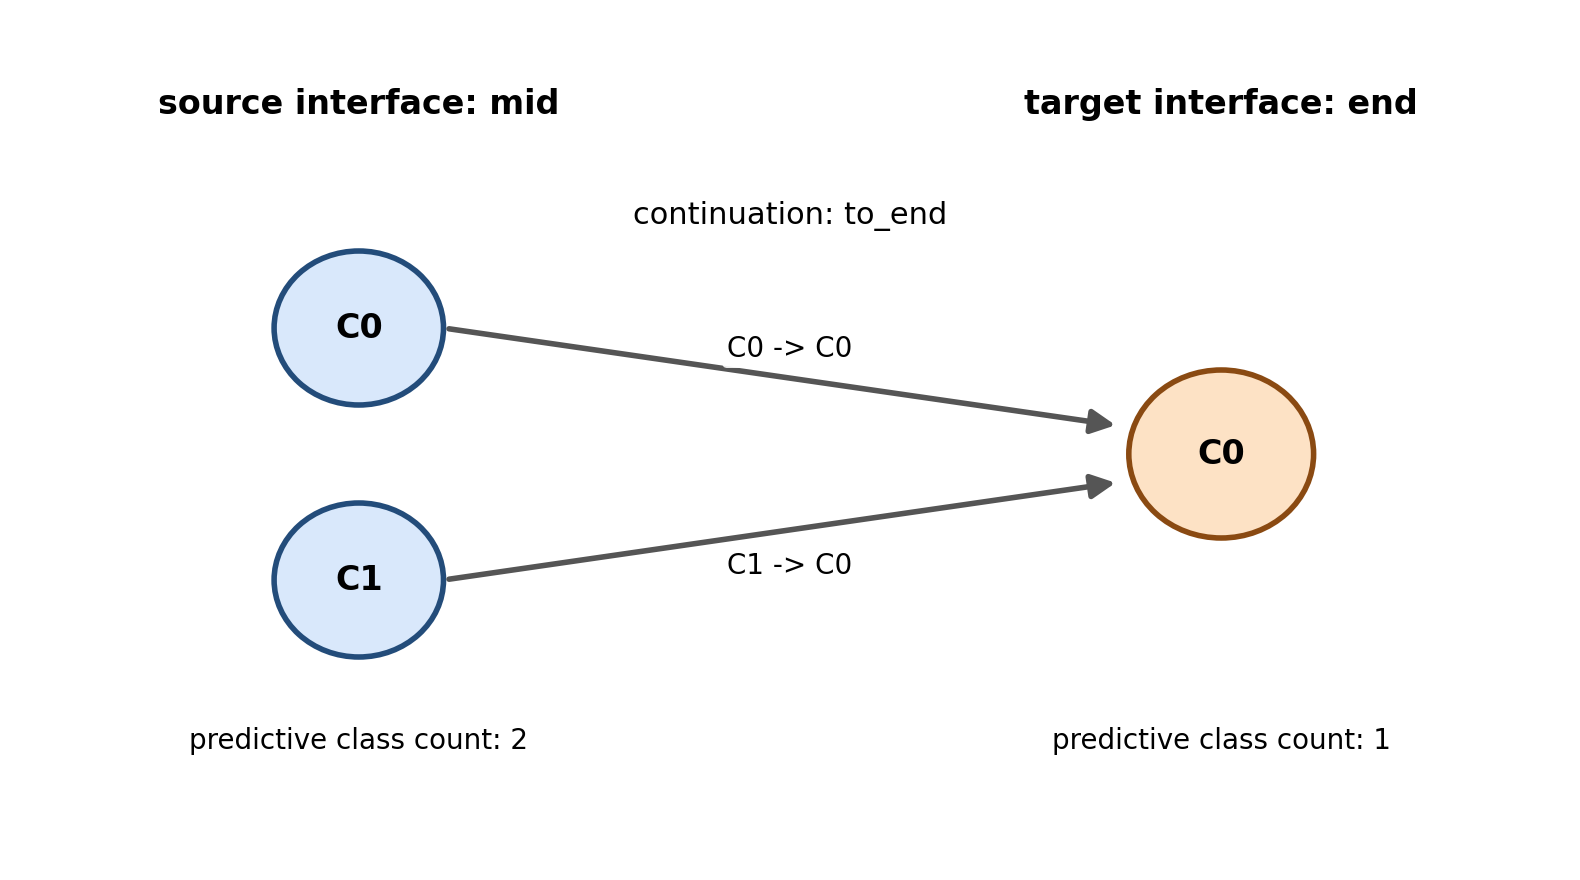
\includegraphics[width=0.82\linewidth]{generated/dissipative_collapse}
\caption{Dissipative transport collapse in the benchmark \texttt{dissipative\_memory}. The source predictive quotient at \texttt{mid} has two classes, while the target predictive quotient at \texttt{end} has one. Under the designated continuation \texttt{to\_end}, both source classes map into the same target class.}
\label{fig:dissipative-collapse}
\end{figure}

\subsection{Memory-wheel benchmark}\label{subsec:bench-memory-wheel}
The memory-wheel benchmark is the principal coherent-memory candidate. At the measured interface \texttt{mid}, the benchmark has $|\CurrentQ|=1$, $|\PredictiveQ|=2$, max fiber size $2$, witness count $1$, exact discrepancy $1$, current loop score $0$, predictive loop score $1$, and class label \texttt{coherent\_candidate}. Thus the benchmark exhibits the full same-now/different-later pattern in one fixed-support object: one current class contains two predictive classes, and the designated loop acts nontrivially only at the predictive level.

The benchmark has no completion or currentization comparison. Both \texttt{flattening\_status} and \texttt{currentization\_status} are \texttt{skipped}. These fields supply no evidence of resistance to repair. The positive evidence is the directly checked witness and swap action, which realize the quotient-level asymmetry pattern. The readout \texttt{to\_end} distinguishes histories in one current class and therefore does not descend to the current quotient; \texttt{swap\_mid} does. The label \texttt{coherent\_candidate} denotes this classical finite observational pattern, not a quantum or irreducibility claim.

The quotient-level asymmetry is explicit. Under the designated loop \texttt{swap\_mid}, the current quotient has one class and is fixed, while the predictive quotient has two classes, $C0$ and $C1$, that are exchanged. The best witness pair is \texttt{h\_mid\_0}, \texttt{h\_mid\_1}, both lying in the same current class but separated predictively by exact discrepancy $1$. Figure~\ref{fig:memory-wheel-asymmetry} summarizes this structure. This is the most direct exact finite realization in the suite of a loop that is trivial on $\CurrentQ$ and nontrivial on $\PredictiveQ$.

\begin{figure}[H]
\centering
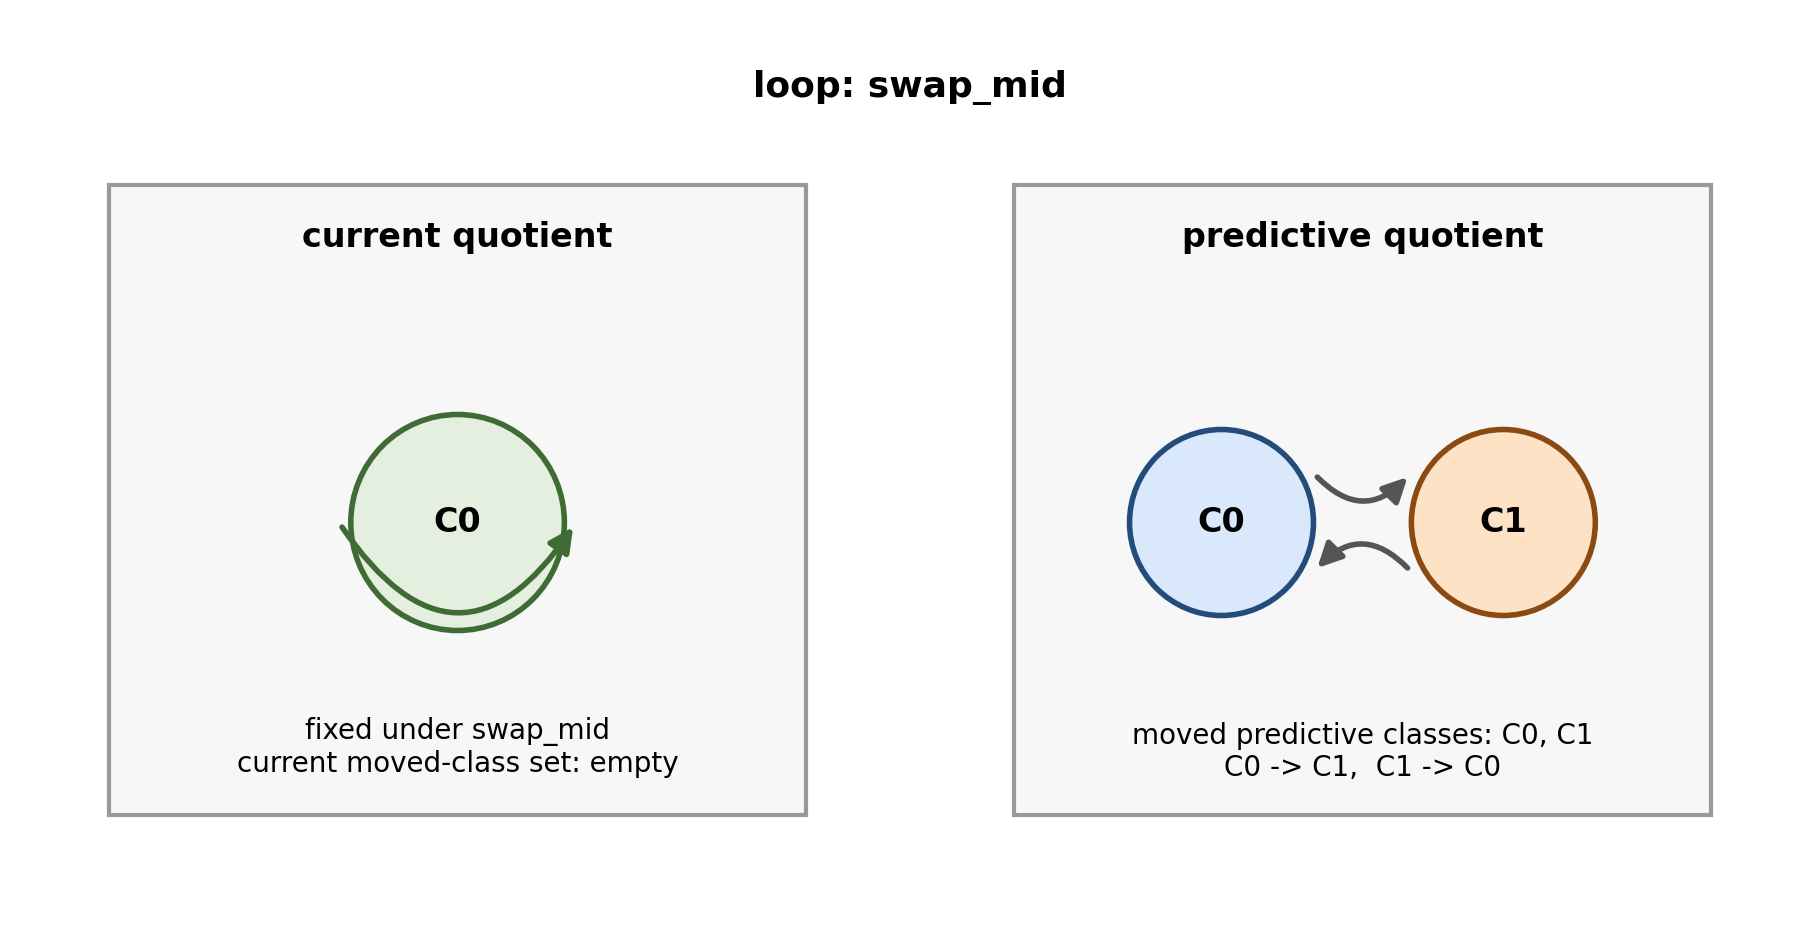
\includegraphics[width=0.88\linewidth]{generated/memory_wheel_asymmetry}
\caption{Loop asymmetry in the benchmark \texttt{memory\_wheel}. At \texttt{mid}, the current quotient has one class and is fixed by \texttt{swap\_mid}, while the predictive quotient has two classes that are exchanged. The moved predictive classes are exactly $C0$ and $C1$, and the current moved-class set is empty.}
\label{fig:memory-wheel-asymmetry}
\end{figure}

\begin{table}[H]
\centering
\caption{Exact metrics for the dissipative and memory-wheel benchmarks.}
\label{tab:bench-flagship-family}
\footnotesize
\setlength{\tabcolsep}{4pt}
\resizebox{\linewidth}{!}{%
\begin{tabular}{@{}llcccccccl@{}}
\toprule
Benchmark & Interface & $|\CurrentQ|$ & $|\PredictiveQ|$ & Max fiber & Wit. & Gap & Cur.\ score & Pred.\ score & Label \\
\midrule
\nolinkurl{dissipative_memory} & \texttt{mid} & 1 & 2 & 2 & 1 & 1 & 0 & 0 & dissipative \\
\nolinkurl{dissipative_memory} & \texttt{end} & 1 & 1 & 1 & 0 & 0 & 0 & 0 & flat \\
\nolinkurl{memory_wheel} & \texttt{mid} & 1 & 2 & 2 & 1 & 1 & 0 & 1 & coherent\_candidate \\
\bottomrule
\end{tabular}}
\end{table}

Taken together, the benchmark suite now exhibits six distinct operational outcomes on fixed support: flat control, artifact trap, flattenable mismatch, explicit latent memory, dissipative collapse, and coherent-candidate loop asymmetry. The next section turns from exemplars to the control and robustness logic that supports those readings.

\section{Controls and Robustness}\label{sec:controls-robustness}
The benchmark labels assigned in Section~\ref{sec:benchmark-suite} do not rest on quotient counts alone. They are supported by explicit paired controls and by bounded perturbation checks carried out on fixed support. This section summarizes that support layer. The purpose is not to claim arbitrary robustness under all possible model changes, but to show that the benchmark readings survive the deterministic perturbation families actually defined for the implementation and that the pairwise labels are tied to explicit admissibility checks rather than informal interpretation.

\subsection{Paired controls}\label{subsec:controls-pairs}
Three paired-control types appear in the benchmark suite, extending the same-support, protocol-trap, and completion logic developed in \citep{Tsiokos2026EventPackages,Tsiokos2026ProtocolTrap,Tsiokos2026FlattenStone}. The first is support fixation: the reported paired interpretations are accompanied by a non-failing comparison of visible support labels. This is a check of the declared comparison surface, not a general certificate that two models are the same physical object. The second is completion or flattening: a raw mismatch is classified as flattenable only when the completed counterpart collapses the predictive residue at the compared interface. The third is currentization: the reported base/refined pair makes the previously hidden distinction current-visible and removes the predictive witness.

The protocol-trap, flattenable, and explicit-latent benchmarks all satisfy these pairwise control conditions in the exact senses recorded by their tracked notes. In the protocol-trap pair, the naive benchmark is non-flat while the honest counterpart is flat, with same-support comparison non-failing. In the flattenable pair, the raw benchmark is non-flat while the completed counterpart collapses the effect and the flattening control records a positive status on the raw side. In the explicit latent pair, the base benchmark is non-flat while the refined same-support counterpart has max fiber size one, zero witnesses, and zero discrepancy, with positive currentization status on the base side. All three conditions are recorded as exact paired readings in the benchmark artifacts.

\subsection{Bounded perturbation robustness}\label{subsec:controls-robustness}
The bounded robustness suite asks a narrower question than generic stability: do the intended benchmark behaviors survive the deterministic perturbation bundles actually attached to the core suite? For the present paper the answer is positive across all seven monitored core benchmarks. In every case, the recorded survival fraction is $1.0$ over $20/20$ perturbation trials, meeting the configured threshold for that benchmark family.

This should be interpreted carefully. The robustness suite does not certify invariance under arbitrary model changes, nor does it substitute for the paired controls described above. It records survival of the named predicates under the configured perturbations. The seven core sweeps each perturb one event weight while leaving the transition kernels and history distributions fixed. Clipping can repeat the base value, and the suite does not require all twenty trial models to be distinct. These are checks of the specified observation perturbations, not of stability under perturbed dynamics. Within the configured perturbation bundles, the flat and honest-control cases remain cleared, the completed and refined counterparts remain collapsed, the dissipative transport pattern persists, and the memory-wheel benchmark retains both witness structure and predictive loop asymmetry.

\begin{table}[H]
\centering
\caption{Core-suite bounded robustness summary.}
\label{tab:robustness-core-suite}
\footnotesize
\setlength{\tabcolsep}{4pt}
\resizebox{\linewidth}{!}{%
\begin{tabular}{@{}llcccc@{}}
\toprule
Benchmark & Predicate & Trials & Passes & Survival & Threshold \\
\midrule
\nolinkurl{flat_control} & \nolinkurl{flat_cleared} & 20 & 20 & 1.0 & 0.95 \\
\nolinkurl{protocol_trap_honest} & \nolinkurl{honest_trap_cleared} & 20 & 20 & 1.0 & 0.95 \\
\nolinkurl{flattenable_completed} & \nolinkurl{completed_collapsed} & 20 & 20 & 1.0 & 0.80 \\
\nolinkurl{latent_memory_base} & \nolinkurl{explicit_latent_base_retains_witness} & 20 & 20 & 1.0 & 0.80 \\
\nolinkurl{latent_memory_refined} & \nolinkurl{explicit_latent_refined_dissolves} & 20 & 20 & 1.0 & 0.80 \\
\nolinkurl{dissipative_memory} & \nolinkurl{dissipative_persists} & 20 & 20 & 1.0 & 0.80 \\
\nolinkurl{memory_wheel} & \nolinkurl{memory_wheel_persists} & 20 & 20 & 1.0 & 0.80 \\
\bottomrule
\end{tabular}}
\end{table}

These controls and robustness results support the benchmark taxonomy but do not enlarge it. In particular, they do not transform a coherent-candidate benchmark into a theorem of stronger physical structure, and they do not turn bounded discovery productivity into a claim of genericity.

\section{Discovery Beyond the Hand-Built Suite}\label{sec:discovery}
The discovery layer tests whether the quotient-level signal isolated by the hand-built suite is confined to a single crafted example. The search spaces are deliberately small, and the resulting atlases should be read as bounded evidence rather than as genericity results. The main findings are that one search space remains all-flat as a control, two search spaces produce non-flat coherent candidates, the shortlisted candidates have distinct descriptor-and-metric signatures under the present dedup audit, and two cyclic exemplars emerge as the strongest bounded follow-up cases.

\subsection{Search spaces and productivity}\label{subsec:discovery-spaces}
Three search spaces were used in the multi-space discovery pass. The first, \nolinkurl{fixed_support_core_small}, functions as a control space and remains all-flat: it evaluates four candidates, all of which are classified \texttt{flat}, with no shortlisted follow-up candidates. The second, \texttt{cyclic\_memory\_small}, is the primary productive search space: it evaluates eight candidates, all classified \texttt{coherent\_candidate}, and yields a combined shortlist of four. The third, \texttt{groupoid\_probe\_small}, is also productive under the present engine: it evaluates eight candidates split between four \texttt{flat} and four \texttt{coherent\_candidate} outcomes, yielding a combined shortlist of three.

The primary-interface comparisons in these tables pass the direct refinement check. However, eight cyclic and four groupoid candidates omit an identity continuation at the terminal interface \texttt{i1}; their terminal future signature is empty, with $|\PredictiveQ|=1$ and $|\CurrentQ|=2$. There is no comparison map induced by refinement at those interfaces. Thus these discovery catalogs are bounded experimental catalogs, not full instances of the abstract identity-and-composition core. No terminal comparison or unrestricted all-future sufficiency claim is inferred from them.

These search results show that the coherent-candidate signal is not confined to the hand-built memory-wheel benchmark and that the discovery machinery also contains an all-flat control space. They do not show that coherent-candidate behavior is generic, exhaustive, or uniformly distributed across search spaces.

\begin{table}[H]
\centering
\caption{Multi-space discovery summary from the tracked discovery note.}
\label{tab:discovery-multispace}
\footnotesize
\setlength{\tabcolsep}{4pt}
\resizebox{\linewidth}{!}{%
\begin{tabular}{@{}lccccccc@{}}
\toprule
Search space & Flat & Dissipative & Coherent & Non-flat & Shortlist & All-flat & Status \\
\midrule
\nolinkurl{fixed_support_core_small} & 4 & 0 & 0 & 0 & 0 & true & control \\
\nolinkurl{cyclic_memory_small} & 0 & 0 & 8 & 8 & 4 & false & productive \\
\nolinkurl{groupoid_probe_small} & 4 & 0 & 4 & 4 & 3 & false & productive \\
\bottomrule
\end{tabular}}
\end{table}

\subsection{Shortlist, bounded robustness, and promoted exemplars}\label{subsec:discovery-shortlist}
The smoke-search shortlist for \texttt{cyclic\_memory\_small} contains four candidates:
\[
\texttt{cand\_0000},\;
\texttt{cand\_0001},\;
\texttt{cand\_0002},\;
\texttt{cand\_0006}.
\]
All four are classified \texttt{coherent\_candidate} and all four pass the bounded shortlisted-candidate robustness check at the configured threshold $0.50$. Their recorded survival fractions are $0.50$, $0.625$, $0.50$, and $0.75$, respectively.

The promoted-exemplar stage then selects two cyclic candidates for follow-up:
\[
\texttt{cyclic\_memory\_small:cand\_0006},
\qquad
\texttt{cyclic\_memory\_small:cand\_0001}.
\]
These are not claimed to be uniquely optimal in any stronger sense than the implemented promotion rule. They are simply the strongest bounded follow-up exemplars under the current ranking, robustness, and distinctness criteria already encoded in the repo.

\begin{table}[H]
\centering
\caption{Promoted discovery exemplars from the tracked exemplar note.}
\label{tab:discovery-exemplars}
\footnotesize
\setlength{\tabcolsep}{4pt}
\begin{tabularx}{\linewidth}{@{}>{\raggedright\arraybackslash}X>{\raggedright\arraybackslash}Xcccc>{\raggedright\arraybackslash}X@{}}
\toprule
Qualified id & Class & Survival & Threshold & \shortstack{Meets\\threshold} & Distinctness & Source space \\
\midrule
\nolinkurl{cyclic_memory_small:cand_0006} & \nolinkurl{coherent_candidate} & 0.75 & 0.50 & true & singleton & \nolinkurl{cyclic_memory_small} \\
\nolinkurl{cyclic_memory_small:cand_0001} & \nolinkurl{coherent_candidate} & 0.625 & 0.50 & true & singleton & \nolinkurl{cyclic_memory_small} \\
\bottomrule
\end{tabularx}
\end{table}

\subsection{Dedup audit and the dropped recombination candidate}\label{subsec:discovery-dedup}
The multi-space dedup audit evaluates the union of the per-space combined shortlists. In the current repo state this audit contains seven shortlisted candidates in total and returns seven singleton clusters. The audit compares declared family descriptors and primary metrics. Its seven singleton clusters mean that none match under those criteria; they do not establish nonisomorphism of the underlying kernels or minimal state machines. This is a useful implementation result, but again a bounded one: it depends on the current search spaces, shortlist rules, and dedup criteria, and it does not by itself imply broad diversity in any stronger external sense.

A final scope boundary concerns the optional relative-route recombination benchmark. That candidate was explored and then dropped. Under the current future-signature semantics, its non-flat behavior reduced to ordinary single-continuation predictive distinctions already captured more cleanly by the existing benchmark family. It is therefore not part of the benchmark suite, not part of the discovery inventory, and not used as evidence in this paper. We record it only as a dropped candidate under the present semantics, not as a negative theorem about richer future extensions.

In summary, the coherent-candidate signal is not confined to a single hand-built benchmark, but it has only been established here in bounded fixed-support search spaces with conservative triage and robustness rules.

\section{Discussion}\label{sec:discussion}
This paper isolates one question: when does route dependence survive below the current event interface as predictive residue? The answer developed here is quotient-level rather than ontological. On fixed support, current-event indistinguishability and future-predictive indistinguishability need not coincide, and the comparison between the resulting quotients organizes both the theorem layer and the exact finite evidence. The benchmark suite, control ledger, robustness suite, and bounded discovery search then show that this distinction is operationally realized.

\subsection{What the paper establishes}\label{subsec:discussion-established}
At the abstract level, the paper defines a quotient-comparison framework. The current quotient $\CurrentQ$ records what is visible at an interface under the present event package, while the predictive quotient $\PredictiveQ$ records what remains relevant for all later admissible observations. The comparison map $\PredictiveQ \to \CurrentQ$ is canonical, predictive transport is well defined, current transport is defined for current-compatible continuations, witness existence is equivalent to strict refinement of that map, and loop action is intertwined by the comparison map. The individual results are standard quotient algebra; the contribution is the choice of definitions and their assembly into a framework for route transport on fixed support.

At the exact finite level, the benchmark suite shows that the quotient comparison supports an operational taxonomy. Flat controls exhibit no hidden predictive residue. The protocol-trap pair shows that route sensitivity can disappear under honest internalization. The flattenable pair shows that some mismatch is removable by admissible completion. The explicit latent pair shows that predictive residue can be real while still becoming current-visible under same-support refinement. The dissipative benchmark shows that predictive distinctions can collapse under later transport. The memory-wheel benchmark then gives the strongest concrete asymmetry in the suite: one current class, two predictive classes, trivial current loop action, and nontrivial predictive loop action.

The robustness and discovery layers strengthen these results in bounded ways. The robustness suite records predicate survival under the configured perturbations; this is not a proof of stability under arbitrary nearby kernels. The discovery searches show that coherent-candidate behavior is not confined to one hand-built example and that the discovery machinery also contains an all-flat control space.

\subsection{Limitations and non-claims}\label{subsec:discussion-limitations}
Beyond the scope boundaries stated in Section~\ref{subsec:intro-scope}, two further limitations deserve mention. The Lean formalization is intentionally partial: it covers the quotient comparison, transport, sufficiency on the reachable image, witness/strict-refinement equivalence, and loop-action asymmetry, but does not yet formalize moved-class sets, cardinality-based nontriviality criteria, or richer action-level invariants. Those omissions do not undermine the present results, but they mark the current boundary of the formal development.

The benchmark and discovery labels should also be read operationally rather than ontologically. In particular, \texttt{coherent\_candidate} is a residual category in the classifier, not a certificate of loop asymmetry: the classifier does not use loop scores in assigning that label. Loop asymmetry is established only by the separately reported current and predictive actions. Neither the label nor those actions force a stronger external state representation.

\subsection{Why the quotient comparison matters}\label{subsec:discussion-why}
With the current quotient and predictive quotient separated, the operational possibilities for route-sensitive effects become explicit. A route-sensitive effect may be absent; it may be an artifact of presentation; it may be removable by admissible completion; it may be currentizable by same-support refinement; it may dissipate under later transport; or it may survive as a loop-level asymmetry visible only at the predictive quotient. These are different outcomes, and the quotient-comparison framework gives them a common language.

That common language is also what unifies the benchmark suite. The protocol-trap, flattenable, explicit-latent, dissipative, and memory-wheel cases are not merely different examples; they occupy different positions in the same quotient-comparison landscape. The map $\PredictiveQ \to \CurrentQ$ and its transport behavior provide the common spine.

At the level of adjacent literatures, the predictive quotient is closest to future-oriented state constructions such as causal states, observable operator models, and predictive state representations \citep{ShaliziCrutchfield2001ComputationalMechanics,Jaeger2000ObservableOperatorModels,LittmanSuttonSingh2002PredictiveRepresentationsState}. The current/future comparison is a refinement between two observation-induced partitions. Bisimulation traditions provide related transition-compatible quotients, with different equivalence criteria \citep{Park1981ConcurrencyAutomata,Milner1989CommunicationConcurrency,LarsenSkou1991BisimulationThroughProbabilisticTesting}. The paper does not claim to subsume those frameworks. Its claim is narrower: on fixed support, one can compare what is visible now with what matters later, and one can separate flat, artifactual, removable, currentizable, dissipative, and loop-asymmetric cases within one operational language.

\section{Conclusion}\label{sec:conclusion}
This paper introduced a fixed-support route-transport framework in which current-event indistinguishability and future-predictive indistinguishability define two distinct quotient states. The resulting current quotient $\CurrentQ$, predictive quotient $\PredictiveQ$, and comparison map $\PredictiveQ \to \CurrentQ$ organize both the abstract theorem layer and the exact finite benchmark layer. On the formal side, standard quotient-algebraic results specialize to this setting to give transport, sufficiency, factorization, witness equivalence, and loop-action intertwining. On the exact finite side, the framework is shown to be non-vacuous: benchmarks instantiate flat, artifact, flattenable, explicit-latent, dissipative, and coherent-candidate regimes on fixed support, with bounded robustness and bounded discovery support.

Relative to the declared tests, the predictive quotient records distinctions hidden at the current interface. A compatible loop can move predictive classes while fixing current classes. Paired controls and transport checks then distinguish effects removed by a specified intervention from those retained or dissipated under the tested continuations. These are operational classifications of the examples, not a general criterion for physical significance.

\appendix

\section{Proof Details and Formal Definitions}\label{app:proof-details}
This appendix records the dependency structure behind the theorem spine stated in Section~\ref{sec:theorem-spine}. The body of the paper states only the quotient-level results needed later; the present appendix makes explicit how those results depend on the underlying definitions.

\subsection{Proof dependency map}\label{appsubsec:proof-dependency-map}
The theorem spine has a strictly layered form.
\begin{enumerate}
\item The refinement theorem depends only on the two equivalence relations and the availability of the identity continuation.
\item Predictive transport depends on the push-composition law; current transport additionally requires current compatibility of the selected continuation. Refinement supplies the comparison map.
\item The future-sufficiency theorem depends only on the definition of future observables and the predictive quotient.
\item The reachable-image factorization theorem depends on future sufficiency and on the fact that equal sufficient-state values force future-predictive equivalence.
\item The witness theorem depends on the quotient comparison map and the correspondence between representative-level inequivalence and quotient-level strict refinement.
\item The loop-asymmetry theorem depends on current compatibility of the selected loop, its induced quotient maps, and their intertwining identity.
\end{enumerate}

The role of this ordering is methodological as well as formal. It isolates which parts of the quotient story are purely abstract, which depend on continuation transport, and which require the additional quotient comparison layer.

\subsection{Definitions used by the theorem spine}\label{appsubsec:proof-definitions}
The abstract route-transport package consists of a fixed support object, a family of interfaces, interface-indexed history sets, typed continuation sets, interface-indexed event sets, and the operations of identity continuation, continuation composition, representative push, and current observation, with the identity and composition laws stated in Section~\ref{sec:route-transport-packages}. Current transport additionally requires compatibility for the selected continuation. The two fundamental equivalence relations are current-event equivalence and future-predictive equivalence. Their quotients define the current quotient $\CurrentQ$ and the predictive quotient $\PredictiveQ$, with canonical comparison map $\pi : \PredictiveQ \to \CurrentQ$ induced by refinement.

The finite implementation of Section~\ref{sec:exact-finite-framework} evaluates declared catalogs. It does not automatically furnish a model of the composition-closed abstract package. Each reported finite quotient map is verified by signature matching and constancy on source classes. Extending a catalog by additional experiments may refine its predictive partition.

\subsection{Quotient-level witness and asymmetry logic}\label{appsubsec:proof-witness-asymmetry}
Two abstract constructions play a special role later in the paper. The first is the predictive witness object: a pair of histories that are current-equivalent but not future-predictively equivalent. The second is loop asymmetry: trivial loop action on $\CurrentQ$ together with nontrivial loop action on $\PredictiveQ$. The witness theorem shows that predictive witnesses are equivalent to strict refinement of $\pi$. The asymmetry theorem then shows that a moved predictive class can project to a fixed current class. These two statements together supply the abstract schema behind the principal benchmark.

\section{Lean Formal Core}\label{app:lean-core}
The formal core of the paper has been mechanized in Lean~4 in the isolated project under \texttt{lean/} \citep{deMouraUllrich2021Lean4}. The formalization is not intended to replace the paper’s mathematical exposition; its role is to anchor the theorem spine and the quotient-comparison layer with machine-checked statements.

\subsection{Lean module layout}\label{appsubsec:lean-layout}
The current Lean modules are:
\begin{itemize}
\item \texttt{lean/HolonomyMemory/Interfaces.lean},
\item \texttt{lean/HolonomyMemory/Equivalences.lean},
\item \texttt{lean/HolonomyMemory/Transport.lean},
\item \texttt{lean/HolonomyMemory/Sufficiency.lean},
\item \texttt{lean/HolonomyMemory/Witnesses.lean},
\item \texttt{lean/HolonomyMemory/Loops.lean},
\item \texttt{lean/HolonomyMemory/Asymmetry.lean},
\item \texttt{lean/HolonomyMemory/Examples.lean}.
\end{itemize}
The root import surface is \texttt{lean/HolonomyMemory.lean}. The isolated build command is
\[
\texttt{cd lean \&\& lake build}.
\]

\subsection{Lean theorem map}\label{appsubsec:lean-theorem-map}
The principal Lean names used in this paper are the following.
\begin{itemize}[leftmargin=*]\small
\item Refinement:
\nolinkurl{futurePredictiveEquiv_implies_currentEventEquiv}

\item Predictive transport:
\nolinkurl{futurePredictiveEquiv_push}

\item Current/predictive comparison under transport:
\nolinkurl{predictiveToCurrent_commutes_with_transport}

\item Future sufficiency:
\nolinkurl{predictiveQuotient_futureSufficient}

\item Kernel refinement from sufficiency:
\nolinkurl{futureSufficient_stateEq_implies_futurePredictiveEquiv}

\item Reachable-image factorization:
\nolinkurl{futureSufficient_factorsThroughPredictiveQuotient_onReachable}

\item Reachable-image uniqueness:
\nolinkurl{futureSufficient_factorization_unique_onReachable}

\item Witness/strict-refinement equivalence:
\nolinkurl{strictRefinement_iff_nonempty_predictiveWitness}

\item Loop-action intertwining:
\nolinkurl{predictiveToCurrent_commutes_with_loopAction}

\item Flagship asymmetry:
\nolinkurl{loopAsymmetry_exhibits_movedPredictive_fixedCurrent}
\end{itemize}

\subsection{Current formal scope}\label{appsubsec:lean-scope}
Current transport and loop commutation now take an explicit \nolinkurl{CurrentCompatible} hypothesis. The two-interface Boolean model in \path{lean/HolonomyMemory/Examples.lean} proves \nolinkurl{bitCore_witness}, \nolinkurl{bitCore_loop_asymmetry}, and \nolinkurl{bitCore_read_not_compatible}; it establishes that the revised assumptions admit witnesses and loop asymmetry. This model is a mechanized illustration, not an import of the JSON benchmark suite. The theorem \nolinkurl{currentEventEquiv_implies_future_of_all_compatible} records why universal current compatibility would collapse the distinction.

The Lean development currently covers the quotient comparison story needed for the paper: equivalence refinement, transport, comparison-map commutation, reachable-image sufficiency and factorization, witness strictness, and loop asymmetry. It does not yet formalize moved-class sets, cardinality-based nontriviality criteria, or richer action-level invariants. Those omissions are real, but they do not undercut any theorem claim made in the main body.

\section{Computational Methods}\label{app:computational-methods}
This appendix records the implementation-facing computational details used by the benchmark, robustness, and discovery layers.

\subsection{Exact finite representation}\label{appsubsec:comp-exact}
All benchmark and discovery models are evaluated as exact finite route-transport packages. Histories are rational distributions on finite internal state sets. Continuations are rational row-stochastic kernels. Event packages are rational functions on visible support labels. Signature computation, partition construction, witness enumeration, transport maps, and loop-action scores are evaluated by exact rational comparison. Perturbation generation and summary serialization use decimal and floating representations in places; exact evaluation applies to the resulting encoded model, not to an idealized real-valued perturbation.

\subsection{Declared catalogs and deterministic order}\label{appsubsec:comp-order}
At each measured interface, current signatures are computed from the declared event package in declared event order. Future signatures are computed from the declared admissible continuation catalog and later event packages in deterministic continuation/event order. No transitive closure is inserted at the signature-construction layer. All quotient sizes, witness counts, and max-fiber values therefore refer to the declared model exactly as encoded in the benchmark or discovery artifact.

\subsection{Diagnostics}\label{appsubsec:comp-diagnostics}
The benchmark and discovery results use four primary diagnostics:
\begin{enumerate}
\item witness count;
\item max fiber size of the comparison map $\PredictiveQ \to \CurrentQ$;
\item exact maximum future gap;
\item loop-action scores on $\CurrentQ$ and $\PredictiveQ$.
\end{enumerate}
The exact maximum future gap is the implementation-facing form of the predictive-sufficiency deficit used in the closure-deficit line of work \citep{Tsiokos2026CastStone}. In the machine-readable outputs the corresponding metric name is \nolinkurl{exact_max_abs_future_gap}.

\subsection{Paired controls}\label{appsubsec:comp-controls}
Three paired-control types are used in the benchmark suite:
\begin{enumerate}
\item support fixation;
\item completion / flattening;
\item currentization.
\end{enumerate}
These controls are implemented as explicit paired comparisons rather than as informal judgment calls. The corresponding artifact fields are \nolinkurl{support_fixation_status}, \texttt{flattening\_status}, and \texttt{currentization\_status}.

\subsection{Bounded robustness}\label{appsubsec:comp-robustness}
Bounded robustness is evaluated by deterministic perturbation bundles that preserve the structural shape of each model while perturbing selected numeric leaves. Probability-bearing vectors and rows are renormalized when required. The benchmark-side robustness suite reports benchmark-specific survival fractions under explicitly named predicates, while the discovery-side shortlisted robustness pass uses a smaller bounded perturbation bundle suitable for triage rather than for benchmark certification.

\subsection{Discovery and triage}\label{appsubsec:comp-discovery}
Discovery proceeds in three stages. First, a search space is enumerated in deterministic order and capped by its configured maximum candidate count. Second, realizable candidates are instantiated into exact finite packages and evaluated into an atlas. Third, productive spaces are triaged into shortlists, optionally followed by bounded shortlisted-candidate robustness, multi-space aggregation, dedup auditing, and exemplar promotion. The search spaces remain deliberately small and should be read as bounded evidence rather than as exhaustive surveys.

\section{Artifact and Figure Source Map}\label{app:artifact-map}
This appendix records the provenance of the tables and figures used in the paper and points to the tracked artifact notes that back the implementation-facing claims. The accompanying repository is available at \url{https://github.com/ioannist/six-birds-route-transport}.

\subsection{Main text tables}\label{appsubsec:artifact-tables}
The tables in the main text draw from the following tracked sources.
\begin{description}[leftmargin=!,labelwidth=2.8cm]\small
\item[Table~\ref{tab:theorem-lean-map}] source files:\\
\path{lean/HolonomyMemory/Equivalences.lean},\\
\path{lean/HolonomyMemory/Transport.lean},\\
\path{lean/HolonomyMemory/Sufficiency.lean},\\
\path{lean/HolonomyMemory/Witnesses.lean},\\
\path{lean/HolonomyMemory/Loops.lean},\\
\path{lean/HolonomyMemory/Asymmetry.lean}.

\item[Table~\ref{tab:bench-control-family}] source notes:\\
\path{docs/results/flat_control.md},\\
\path{docs/results/protocol_trap_naive.md},\\
\path{docs/results/protocol_trap_honest.md},\\
\path{docs/results/flattenable_raw.md},\\
\path{docs/results/flattenable_completed.md},\\
\path{docs/results/latent_memory_base.md},\\
\path{docs/results/latent_memory_refined.md}.

\item[Table~\ref{tab:bench-control-pairs}] source notes:\\
\path{docs/results/protocol_trap_pair.md},\\
\path{docs/results/flattenable_pair.md},\\
\path{docs/results/latent_memory_pair.md}.

\item[Table~\ref{tab:bench-flagship-family}] source notes:\\
\path{docs/results/dissipative_memory.md},\\
\path{docs/results/memory_wheel.md}.

\item[Table~\ref{tab:robustness-core-suite}] source note:
\path{docs/results/robustness_core_suite.md}.

\item[Table~\ref{tab:discovery-multispace}] source note:
\path{docs/results/multi_space.discovery.md}.

\item[Table~\ref{tab:discovery-exemplars}] source note:
\path{docs/results/discovery_exemplars.md}.
\end{description}

\subsection{Main text figures}\label{appsubsec:artifact-figures}
The figures in the main text are paper-local renderings of tracked benchmark results.
\begin{description}[leftmargin=!,labelwidth=2.8cm]
\item[Figure~\ref{fig:dissipative-collapse}] source note:
\path{docs/results/dissipative_memory.md}; paper-local file:
\path{paper/figures/generated/dissipative_collapse.png}.

\item[Figure~\ref{fig:memory-wheel-asymmetry}] source note:
\path{docs/results/memory_wheel.md}; paper-local file:
\path{paper/figures/generated/memory_wheel_asymmetry.png}.
\end{description}

\subsection{Aggregate and discovery support artifacts}\label{appsubsec:artifact-support}
The broader implementation-facing support for the paper is collected in the following machine-readable artifacts:
\begin{itemize}[leftmargin=*]
\item \path{artifacts/results/benchmark_suite.json},
\item \path{artifacts/results/robustness/core_suite.robustness.json},
\item \path{artifacts/results/discovery/multi_space.discovery.json},
\item \path{artifacts/results/discovery/multi_space.dedup.json},
\item \path{artifacts/results/discovery/promoted_exemplars.json},
\item \path{artifacts/results/aggregate_outputs.json},
\item \path{artifacts/results/aggregate_figures.json}.
\end{itemize}
These are not substitutes for the paper's claims, but they are the machine-readable source layer from which the tracked notes and summary tables are built.

\section{Reproducibility Note}\label{app:reproducibility}
The repo includes a reproducibility freeze and a small fixed command surface for rerunning the implementation. The four frozen commands are:
\begin{itemize}
\item \texttt{make test},
\item \texttt{make benchmark-suite},
\item \texttt{make discovery-smoke},
\item \texttt{make lean-build}.
\end{itemize}
The benchmark-side top-level outputs are:
\begin{itemize}
\item \nolinkurl{artifacts/results/benchmark_suite.json},
\item \nolinkurl{artifacts/tables/benchmark_suite.csv},
\item \nolinkurl{docs/results/benchmark_suite.md}.
\end{itemize}
The discovery-side top-level outputs are:
\begin{itemize}
\item \nolinkurl{artifacts/results/discovery/discovery_smoke.json},
\item \nolinkurl{docs/results/discovery_smoke.md}.
\end{itemize}
The Lean build is isolated under \texttt{lean/} and is reproduced by
\[
\texttt{cd lean \&\& lake build}.
\]

A machine-readable freeze summary is recorded in
\nolinkurl{artifacts/results/repro_freeze.json}, and the operational command summary is recorded in
\texttt{docs/ops/reproducibility.md}. The results reported in the present paper are intended to be traceable to those fixed commands and tracked artifacts.

\bibliographystyle{plainnat}
\bibliography{references}

\end{document}
